\documentclass[a4paper]{article}
\usepackage[pdftex]{graphicx}
\usepackage[utf8]{inputenc}
\usepackage{enumerate}
\usepackage{icomma}
\usepackage{siunitx}
\sisetup{locale=DE} 
\usepackage{amssymb}
\usepackage{tikz}
\usepackage{href-ul}
\hypersetup{
	colorlinks=true,
	linkcolor=blue,
	urlcolor=blue}
\usepackage{geometry}
\geometry{a4paper, top=15mm, left=15mm, right=15mm, bottom=15mm,
	headsep=10mm, footskip=12mm}

\begin{document}
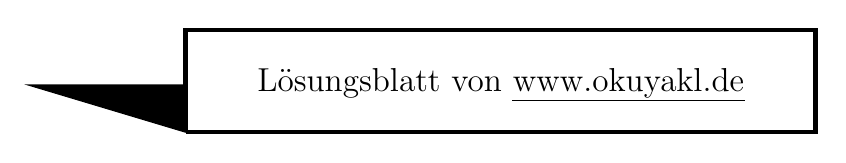
\begin{tikzpicture}(10,3)
	\draw[ultra thick](2,0) --(10,0) -- (10,1.3) --(2,1.3) -- (2,0);
	\draw[fill=black](2,0)-- (0,.6) -- (2,.6) -- (2,0);
	\node at (6,.6) {\large Lösungsblatt von \href{https://www.okuyakl.de}{www.okuyakl.de}};
\end{tikzpicture}
\vspace{0.5 cm}

\noindent{\bf Aufgabe 1.}\\
Wir berechnen zuerst $r$:
$$A={ b \cdot r\over 2} \quad \Rightarrow \quad r = { 2A \over  b }= {2\cdot \SI{12,5}{\centi\meter^2} \over  \SI{8}{\centi\meter}}=\SI{3,125}{\centi\meter}$$
Weiter gilt für den Mittelpunktswinkel:
$$b={\mu \over 180^{\circ}}\cdot \pi r   \quad \Rightarrow \quad \mu = {180^{\circ}\cdot b \over \pi r} = 147^\circ$$  

\noindent{\bf Aufgabe 2.}\\
Der Flächeninhalt ist ein Viertelkreis mit Radius $a$ minus einen Halbkreis mit Radius $a/2$:
$$A={1\over 4} \cdot \pi a^2-{1\over 2} \cdot \pi \left({a\over 2}\right)^2 = {1\over 8}\cdot \pi a^2 ={1\over 8}\cdot \pi \cdot (\SI{5}{\centi\meter})^2 = \SI{9,82}{\centi\meter^2}$$
Der Umfang setzt sich zusammen aus dem Umfang eines Halbkreises mit Radius $a/2$, dem Umfang eines Viertelkreises mit Radius $a$ und der Länge $a$:
$$U= \pi \cdot {a\over 2} + {\pi \over 2} \cdot a + a = \pi \cdot a + a = \SI{20,7}{\centi\meter}$$

\noindent{\bf Aufgabe 3.}\\
Wir zerlegen die Figur in Teilfiguren:
\begin{itemize}
	\item 2 Halbkreise mit dem Radius $a$; Fläche $A_{HK}$
	\item ein Quadrat mit der Seitenlänge $2a$; Fläche $A_{Q}$
	\item ein Dreieck mit der Grundlinie $2a$ und der Höhe $a$; Fläche $A_{Dr}$
\end{itemize}   
Die Flächeninhalte der Teilfiguren werden addiert:
$$A_{ges}=2\cdot A_{HK} + A_{Q} + A_{Dr} = 2\cdot {1\over 2} \pi a^2 + 4a^2 + {1\over 2}\cdot 2 a\cdot a = \pi a^2 + 5a^2 = a^2(5+\pi)$$

\noindent
\fbox{
	\begin{minipage}{0.47\textwidth}
	\noindent {\bf Aufgabe 4. i)}\\	
	$$\alpha_{RAD}={225^\circ \over 180^\circ}\cdot \pi ={5\over 4}\pi$$
	\end{minipage}
}
\fbox{
	\begin{minipage}{0.47\textwidth}
	\noindent {\bf Aufgabe 4. ii)}\\
	$$\alpha_{RAD}={100^\circ \over 180^\circ}\cdot \pi ={5\over 9}\pi$$	
	\end{minipage}
}
\fbox{
	\begin{minipage}{0.47\textwidth}
	\noindent {\bf Aufgabe 4. iii)}\\
	$$\alpha_{DEG}=0,8 \cdot {180^\circ \over \pi} = 45,84^\circ$$ 
	\end{minipage}
}
\fbox{
 	\begin{minipage}{0.47\textwidth}
 	\noindent {\bf Aufgabe 4. iv)}\\
 	$$\alpha_{DEG}={7\over 4}\pi \cdot {180^\circ \over \pi} = 315^\circ$$ 	
 	\end{minipage}
 }
\vspace{0,5 cm}

\noindent {\bf Aufgabe 5.}\\
$$
\renewcommand{\arraystretch}{2}
\begin{array}{|c|c|c|c|}
\hline
\qquad \mu \qquad & \qquad r \qquad &\qquad b\qquad & \qquad A_S \qquad \\
\hline
50^\circ & \SI{2,3}{\deci\meter} & \SI{2,0}{\deci\meter} & \SI{2,3}{\deci\meter^2} \\
\hline
127^\circ & \SI{4,5}{\centi\meter} & \SI{10}{\centi\meter} & \SI{22,4}{\centi\meter^2}\\
\hline
130^\circ & \SI{8,13}{\milli\meter} & \SI{18,5}{\milli\meter} & \SI{75}{\milli\meter^2} \\
\hline
\end{array}
$$
\begin{center}
	\includegraphics[width=7 cm]{../../viecher/endcomic.pdf}
	
	Hier geht es zurück zum \href{https://www.okuyakl.de/math/m10kreiaL026/aa026.pdf}{Aufgabenblatt}
\end{center}

\end{document}

